\documentclass[a4paper,twoside,11pt]{article}
\usepackage{a4wide,graphicx,fancyhdr,amsmath,amssymb,placeins}
\usepackage{listings}
\usepackage{color}
\usepackage{enumitem}
\usepackage{amsmath}
\usepackage{textcomp}
\usepackage{caption,subcaption}

%----------------------- Macros and Definitions --------------------------

\setlength\headheight{20pt}
\addtolength\topmargin{-10pt}
\addtolength\footskip{20pt}

\newcommand{\N}{\mathbb{N}}
\newcommand{\ch}{\mathcal{CH}}
\newcommand{\cpp}{{\tt C++} }

\newcommand{\solution}[1]{\noindent{\bf Solution to Exercise #1:}}

\renewcommand{\lstlistingname}{Codeblock}
\captionsetup[lstlisting]{font={small,tt}}

\fancypagestyle{plain}{%
\fancyhf{}
\fancyhead[LO,RE]{\sffamily\bfseries\large technische universiteit eindhoven}
\fancyhead[RO,LE]{\sffamily\bfseries\large 2IW02 RTSD}
\fancyfoot[LO,RE]{\sffamily\bfseries\large department of mathematics and computer science}
\fancyfoot[RO,LE]{\sffamily\bfseries\thepage}
\renewcommand{\headrulewidth}{0pt}
\renewcommand{\footrulewidth}{0pt}
}

\pagestyle{fancy}
\fancyhf{}
\fancyhead[RO,LE]{\sffamily\bfseries\large technische universiteit eindhoven}
\fancyhead[LO,RE]{\sffamily\bfseries\large 2IW02 RTSD}
\fancyfoot[LO,RE]{\sffamily\bfseries\large department of mathematics and computer science}
\fancyfoot[RO,LE]{\sffamily\bfseries\thepage}
\renewcommand{\headrulewidth}{1pt}
\renewcommand{\footrulewidth}{0pt}

%-------------------------------- Title ----------------------------------

\title{\vspace{-\baselineskip}\sffamily\bfseries Exercise 1}
\author{
	Rick Veens \qquad Studentno: 0912292\\
	\texttt{r.veens@student.tue.nl}
	\and
	Huib Donkers \qquad Studentno: 0769015\\
	\texttt{h.t.donkers@student.tue.nl}
}

\date{\today}

\definecolor{listinggray}{gray}{0.9}
\definecolor{lbcolor}{rgb}{0.9,0.9,0.9}
\lstset{
backgroundcolor=\color{lbcolor},
    tabsize=4,    
%   rulecolor=,
    language=[GNU]C++,
        basicstyle=\scriptsize,
        upquote=true,
        aboveskip={1.5\baselineskip},
        columns=fixed,
        showstringspaces=false,
        extendedchars=false,
        breaklines=true,
        prebreak = \raisebox{0ex}[0ex][0ex]{\ensuremath{\hookleftarrow}},
        frame=single,
        numbers=left,
        showtabs=false,
        showspaces=false,
        showstringspaces=false,
        identifierstyle=\ttfamily,
        keywordstyle=\color[rgb]{0,0,1},
        commentstyle=\color[rgb]{0.026,0.112,0.095},
        stringstyle=\color[rgb]{0.627,0.126,0.941},
        numberstyle=\color[rgb]{0.205, 0.142, 0.73},
%        \lstdefinestyle{C++}{language=C++,style=numbers}’.
}

% geen stomme indents bij \par
\setlength{\parindent}{0cm}

%--------------------------------- Text ----------------------------------

\begin{document}
\maketitle

\section{}
\subsection{}
\subsubsection{}
We modelled the deadlock free system as show in figure~\ref{fig:SystemDF}, and the deadlocked system as shown in figure~\ref{fig:SystemDC}. As expected, FDR accepts the deadlock free system (firgure~\ref{fig:FDR_DF}), but not the deadlocked system (figure~\ref{fig:FDR_DC}).
\begin{figure}
 \centering
 \begin{subfigure}{\textwidth}
  \centering
  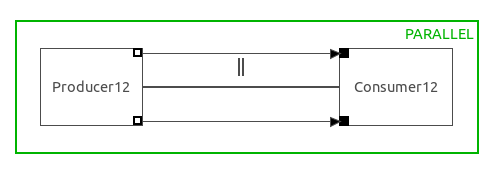
\includegraphics[scale=0.8]{./images/1_1-SystemDF_main.png}
  \caption{Composition of the Producer and Consumer processes.}
 \end{subfigure}
 \begin{subfigure}{0.5\textwidth}
  \centering
	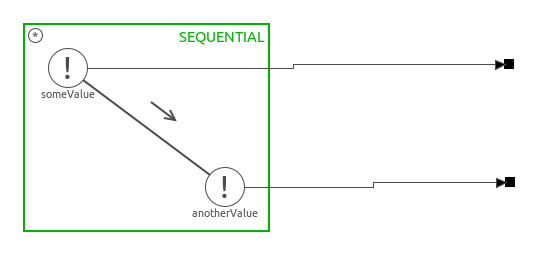
\includegraphics[scale=0.8]{./images/1_1-SystemDF_prod.png}
	\caption{The producer process.}
 \end{subfigure}%
 \begin{subfigure}{0.5\textwidth}
  \centering
	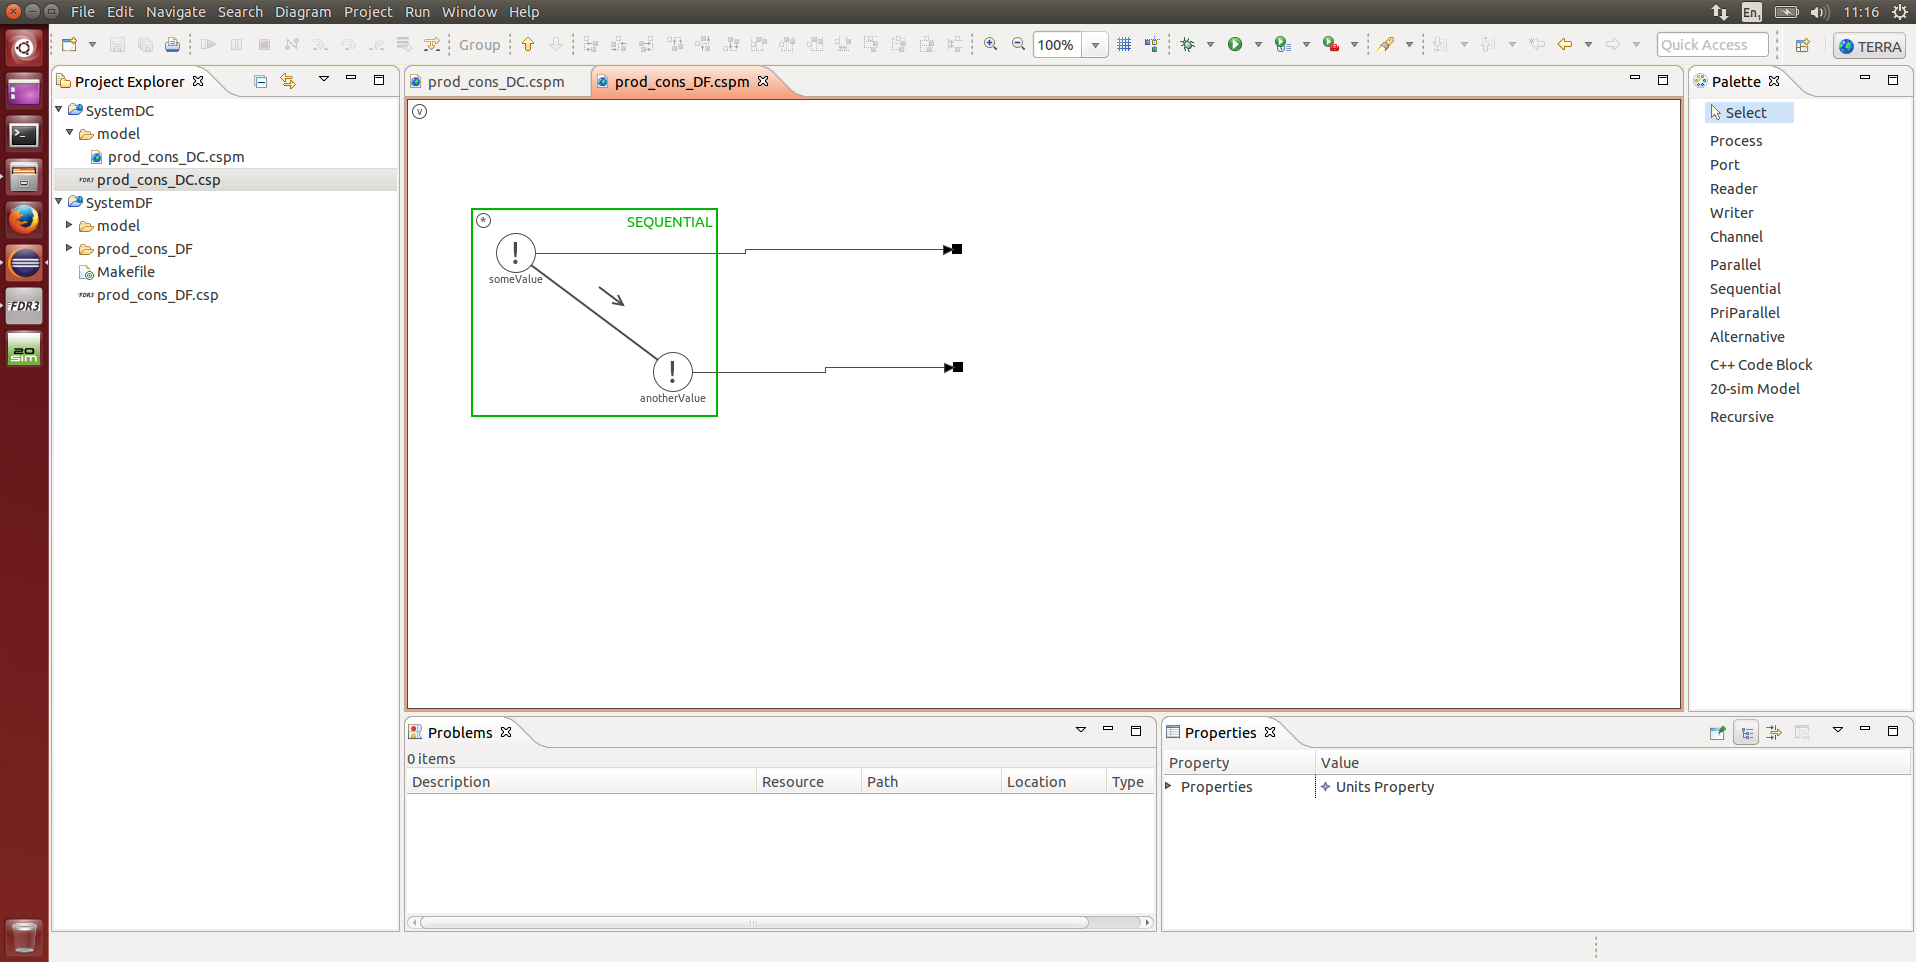
\includegraphics[scale=0.8]{./images/1_1-SystemDF_cons.png}
	\caption{The consumer process.}
 \end{subfigure}
 \caption{The producer-consumer (DF) model.}
 \label{fig:SystemDF}
\end{figure}

\begin{figure}
 \centering
 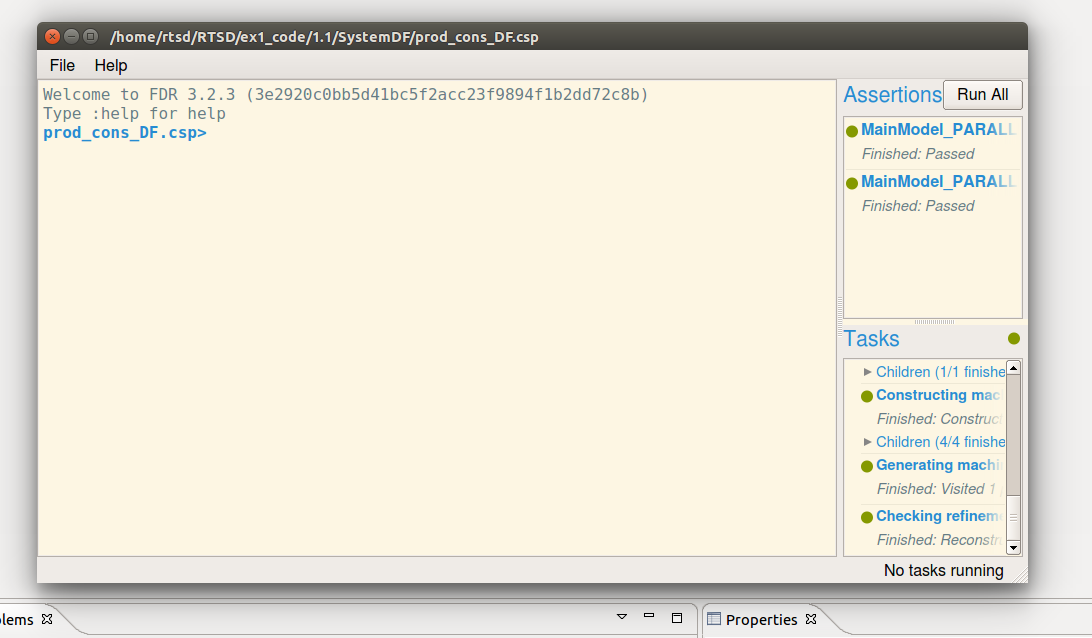
\includegraphics[width=\textwidth]{./images/1_1-SystemDF.png}
 \caption{Successfully passes tests in FDR.}
 \label{fig:FDR_DF}
\end{figure}


\begin{figure}
 \centering
 \begin{subfigure}{\textwidth}
  \centering
  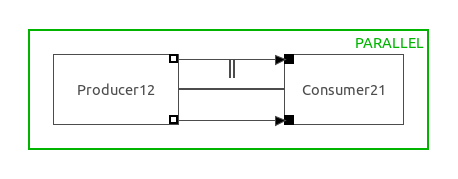
\includegraphics[scale=0.8]{./images/1_1-SystemDC_main.png}
  \caption{Composition of Producer and Consumer processes.}
 \end{subfigure}
 \begin{subfigure}{0.5\textwidth}
  \centering
	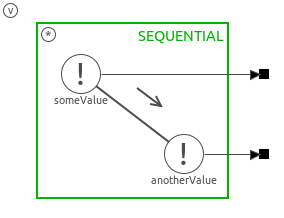
\includegraphics[scale=0.8]{./images/1_1-SystemDC_prod.png}
	\caption{The producer process.}
 \end{subfigure}%
 \begin{subfigure}{0.5\textwidth}
  \centering
	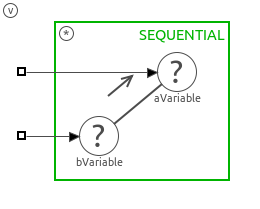
\includegraphics[scale=0.8]{./images/1_1-SystemDC_cons.png}
	\caption{The consumer process.}
 \end{subfigure}
  \caption{The producer-consumer (DC) model.}
  \label{fig:SystemDC}
\end{figure}

\begin{figure}
 \centering
 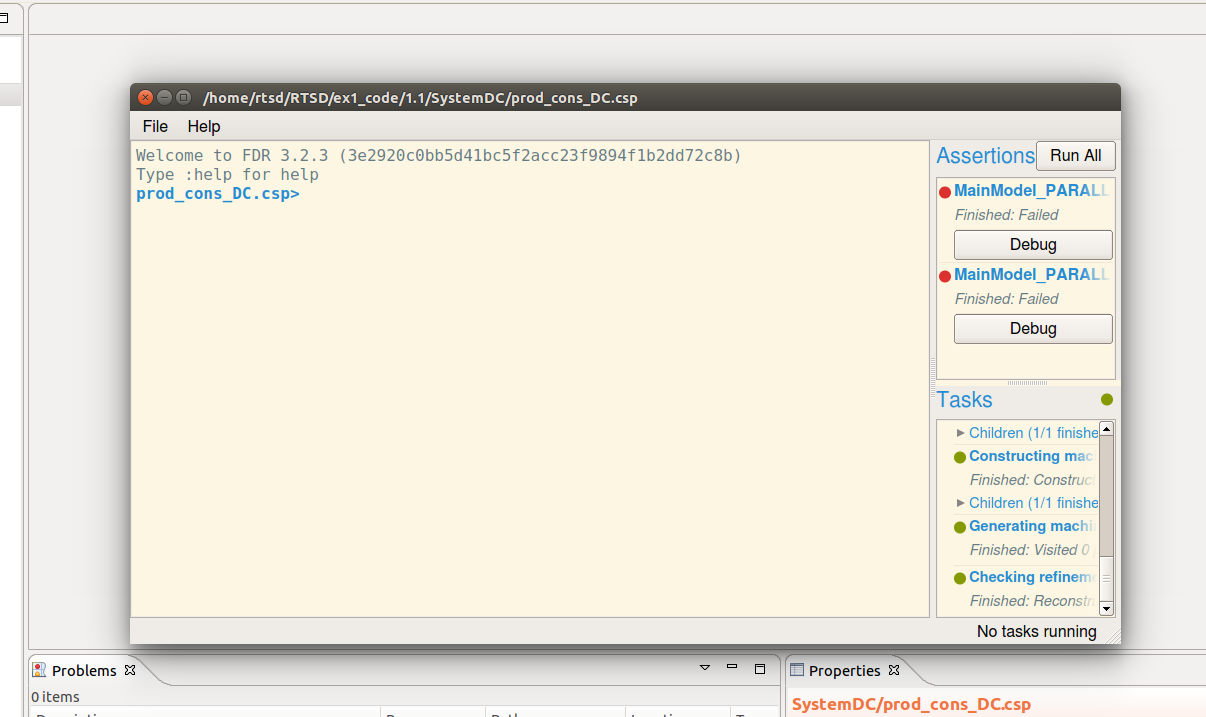
\includegraphics[width=\textwidth]{./images/1_1-SystemDC.png}
 \caption{Fails the tests in FDR.}
 \label{fig:FDR_DC}
\end{figure}

\FloatBarrier
\subsubsection{}
We extended the producer consumer (DF) model from figure~\ref{fig:SystemDF} with code blocks, and added \cpp implementation. The extended model is shown in figure~\ref{fig:SystemDF+} and the code in included in blocks \ref{code:1_2consumer} and \ref{code:1_2producer}. The initial few lines of the output is shown in figure~\ref{fig:SystemDF+_output}.

\begin{figure}
 \centering
 \begin{subfigure}{\textwidth}
  \centering
  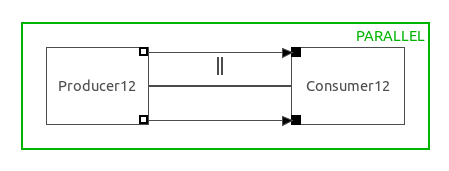
\includegraphics[scale=0.8]{./images/1_2-SystemDF+_main.png}
  \caption{Overview diagram of the producer consumer system.}
 \end{subfigure}
 \begin{subfigure}{0.5\textwidth}
  \centering
	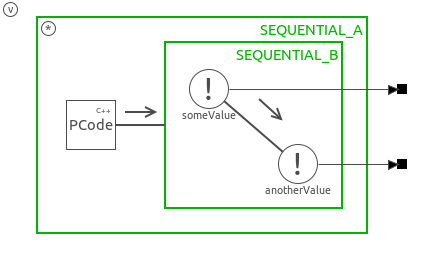
\includegraphics[width=\textwidth]{./images/1_2-SystemDF+_prod.png}
	\caption{The producer process.}
 \end{subfigure}%
 \begin{subfigure}{0.5\textwidth}
  \centering
	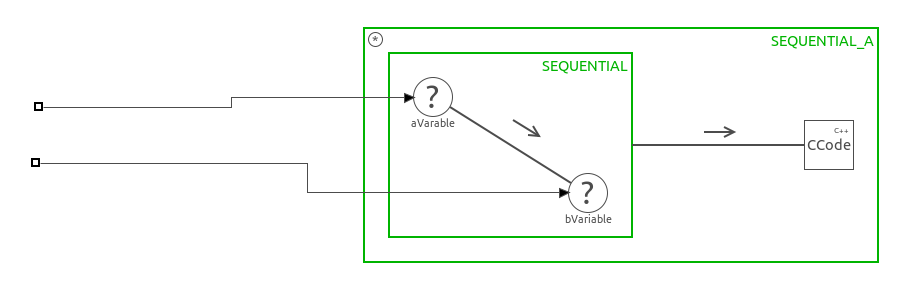
\includegraphics[width=\textwidth]{./images/1_2-SystemDF+_cons.png}
	\caption{The consumer process.}
 \end{subfigure}
 \caption{The producer-consumer (DF) model extended with code.}
 \label{fig:SystemDF+}
\end{figure}

\begin{lstlisting}[caption=Consumer12/CCode.cpp, label=code:1_2consumer, language=C++]
/**
 * Source file for the CCode model
 * Generated by the TERRA CSPm2LUNA generator version 1.1.1
 *
 * protected region document description on begin
 *
 * protected region document description end
 */

#include "Consumer12/CCode.h"
// protected region additional headers on begin
// Each additional header should get a corresponding dependency in the Makefile
// protected region additional headers end

namespace MainModel { namespace Consumer12 { namespace CCode { 

CCode::CCode(int &CCode_aVariable, int &CCode_bVariable) :
    CodeBlock(), CCode_aVariable(CCode_aVariable), CCode_bVariable(CCode_bVariable){
  SETNAME(this, "CCode");

  // protected region constructor on begin
  // protected region constructor end
}

CCode::~CCode()
{
  // protected region destructor on begin
  // protected region destructor end
}

void CCode::execute()
{
  // protected region execute code on begin
	if (this->CCode_aVariable == -1 || this->CCode_bVariable == -1)
		exit();
	else {
		printf("Receiving: CCode_aVariable: \t'%c'\n", this->CCode_aVariable);
		printf("Receiving: CCode_bVariable: \t'%c'\n", this->CCode_bVariable);

		printf("\n");
	}
  // protected region execute code end
}

// protected region additional functions on begin
// protected region additional functions end

// Close namespace(s)
} } } 
\end{lstlisting}


\begin{lstlisting}[caption=Producer12/PCode.cpp, label=code:1_2producer, language=C++]
/**
 * Source file for the PCode model
 * Generated by the TERRA CSPm2LUNA generator version 1.1.1
 *
 * protected region document description on begin
 *
 * protected region document description end
 */

#include "Producer12/PCode.h"
#include "string.h"
// protected region additional headers on begin
// Each additional header should get a corresponding dependency in the Makefile
// protected region additional headers end

namespace MainModel { namespace Producer12 { namespace PCode { 

PCode::PCode(int &PCode_anotherValue, int &PCode_someValue) :
    CodeBlock(), PCode_anotherValue(PCode_anotherValue), PCode_someValue(PCode_someValue){
  SETNAME(this, "PCode");

  // protected region constructor on begin
  // protected region constructor end
}

PCode::~PCode()
{
  // protected region destructor on begin
  // protected region destructor end
}

void PCode::execute()
{
  // protected region execute code on begin

	static int index = 0;

	char *stuff = "Appelflap";

	if (index == strlen(stuff)) {
		this->PCode_someValue = -1;
		this->PCode_anotherValue = -1;
	} else {
		this->PCode_someValue = stuff[index];
		this->PCode_anotherValue = stuff[index++];

		printf("Sending: PCode_someValue: \t'%c'\n", this->PCode_someValue);
		printf("Sending: PCode_anotherValue: \t'%c'\n", this->PCode_anotherValue);
	}


  // protected region execute code end
}

// protected region additional functions on begin
// protected region additional functions end

// Close namespace(s)
} } } 
\end{lstlisting}

\begin{figure}
 \centering
 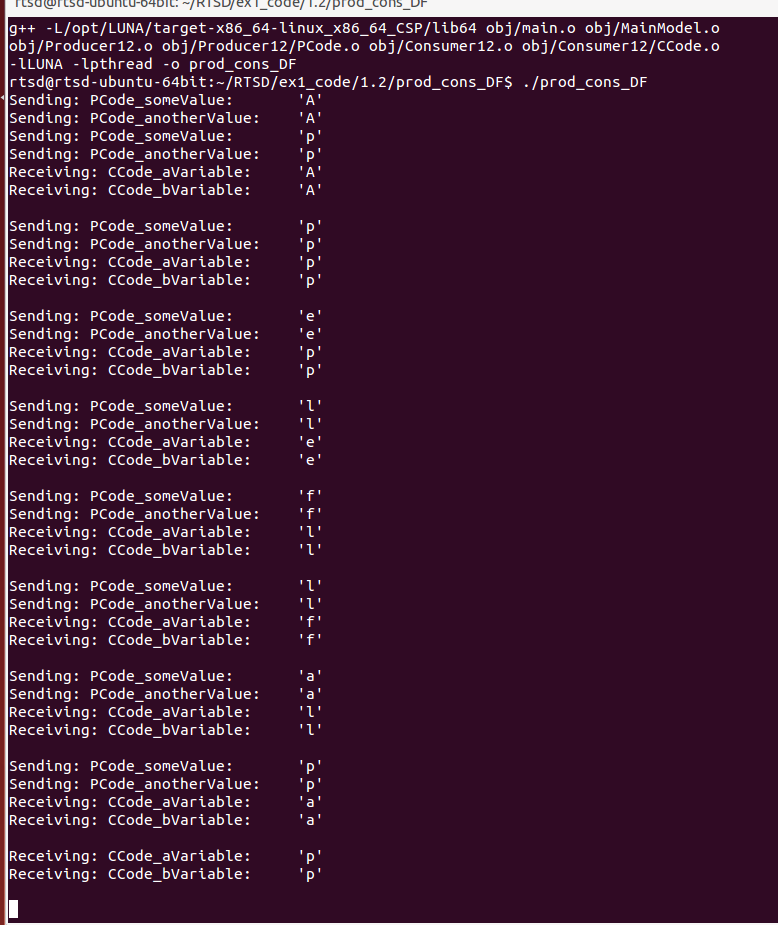
\includegraphics[width=\textwidth]{./images/1_2-SystemDF+_output.png}
 \caption{The output that our system produces.}
 \label{fig:SystemDF+_output}
\end{figure}
\FloatBarrier
\subsubsection{}
The consumer process cannot start before something is written on the channels. The producer process can start with the execution of its \cpp code. The parallel composition of the two processes can therefor only start with the execution of the \cpp code of the producer, hence the first two lines of the output originate from the producer.

Now, for the first channel, both the reader and the writer are available, and no other actions can be done by either process. The data is sent over the channel. After that, the same goes for the second channel.

Next, the producer can start over, starting with the execution of the \cpp code, but now the consumer can also execute its \cpp code. We expect either two lines of output produced by the producer's \cpp code, or two lines produced by the consumers \cpp code. And indeed we see the output of the producer's \cpp code.

Next, the writers in the producer cannot write to the channels, because the readers of the consumer are not ready. First the consumer's \cpp code needs to be executed before the process can recur and execute its readers. Hence the next two lines are produced by the consumer.

Now, the readers and writers do their thing and, again, either the producer's \cpp code can be executed, or the consumer's. We see for the complete initial part of the run that the producer's \cpp code is executed before the consumer's \cpp code.

\subsubsection{}
ProBE is an interpreter for CSPm scripts, the user can manually inspect the possible execution paths. When a process is deadlock free, its execution paths are infinite. ProBE will never see the end of these executionpaths, nor will it know whether it has an end. FDR recognises this infinite behaviour, or rather, it recognises finite behaviour. When it finds the process is able to terminate, it shows that the process fails the deadlock free-test. Similarly it can check for other properties without needing to simulate the complete execution paths likes ProBE does. ProBE can be used to inspect how a process deadlocks.

\subsubsection{}
If we adapt the \cpp code of the producer to start at the beginning of the word again when all characters have been sent, we can observe the behaviour of the process when it runs for a while. We saw previously that the consumer only continued when the producer had to wait. This does not seem fair parallel. But when we watch what happens when the code runs for a while, we occasionally see the consumer receiving four values in a row, meaning that its \cpp code executed before the producer's \cpp code could prepare the next two values for the writers. So when both processes can execute, the parallel composition does not consistently execute one of them before the other. This seems fair.


\subsubsection{}
The composition $A ||| B$ does not deadlock. Whichever process gets to execute its \cpp code first, it will need to wait for the other process directly after. When both have executed their \cpp code, execution can continue by writing and reading on the channels. At no point do the processes wait for the other.

\FloatBarrier
\subsection{}
\FloatBarrier
\subsubsection{}
See Figure~\ref{fig:2_1-model} for some screenshots of the model.
We chose to implement three channels.

\subsubsection{}
See Codeblock~\ref{code:2_1PCode} for the code of \cpp code block PCode. The other code blocks in the program are of no interest, because they merely print their input variable.
\smallskip

Figure~\ref{fig:2_1-output} shows some of the output of the program after extending it with \cpp code.

The decision was made to have the program send each of the three values once. 
After sending the prompt appears again.

The guards on the producer side (see Figure~\ref{fig:2_1-model:producer}) are configured 
in the model in such a way that a value `1' gets send to channel 1, value `2' to channel 2 and value `3' to channel 3.
Any other value that is entered will result in the ``Prullenbak'' \cpp code being executed.

Note that some of the messages are out of order, the same stuff is happening as discussed in exercise 1.1.3.

In short, order we see occurs because the top producer and consumer process are linked in parallel.
The communication of the consumer/producer processes are synchronized, but not the code being executed in their internal \cpp code blocks.

\subsubsection{}
Note that in Figure~\ref{fig:2_1-model:producer} a \cpp codeblock is added called ``Prullenbak''.
This ``Prullenbak'' \cpp code block is executed only when none of the other guard expressions in the ALTERNATIVE block apply.
The function of ``Prullenbak'' is to catch and print input data that is not to be send to the consumer, it is a garbage can.


\subsubsection{}
It is wise to start with the process-structure before implementing \cpp code.

Generally, if you have to choose, you want most of the functionality in the model instead of in \cpp code blocks.
The model also serves as documentation. Making sure the model is of decent quality first helps in containing most of the functionality in the model instead of the \cpp code.

\subsubsection{}
The method we chose to implement is to add another guard that is triggered when none of the other guards are triggered. It is a garbage bin exit.
\smallskip

Another possible method is to copy the guard logic of the alternative blocks in the producer to the ``PCode'' \cpp code block, 
and do a check on the input data to make sure it it checks out with your guard logic.
This idea is less desired, because now you have the guard logic in \emph{two} places: in the model and in the \cpp code.

You could also remove the alternative structure, have only one instead of three channels, and put all your guard logic in the first \cpp code block (PCode).
This idea makes the program harder to understand, so not recommended.

\begin{lstlisting}[caption=Producer/PCode.cpp, label=code:2_1PCode, language=C++]
/**
 * Source file for the PCode model
 * Generated by the TERRA CSPm2LUNA generator version 1.1.1
 *
 * protected region document description on begin
 *
 * protected region document description end
 */

#include "Producer/PCode.h"
// protected region additional headers on begin
#include <stdio.h>
#include <iostream>
#include <algorithm>
// Each additional header should get a corresponding dependency in the Makefile
// protected region additional headers end

namespace MainModel { namespace Producer { namespace PCode { 

PCode::PCode(int &peer) :
    CodeBlock(), peer(peer){
  SETNAME(this, "PCode");

  // protected region constructor on begin
  // protected region constructor end
}

PCode::~PCode()
{
  // protected region destructor on begin
  // protected region destructor end
}

void PCode::execute()
{
  // protected region execute code on begin
	static int index = 3;

	if (index > 2) {
		index = 0;
		while (!initialize()) {
			printf("Numbers not distinct.\n");
		}
	}
	printf("P1->Sending %d\n", vars[index]);
	this->peer = vars[index++];
  // protected region execute code end
}

// protected region additional functions on begin
bool PCode::initialize(void)
{
	printf("Enter 3 numbers\n");
	while (scanf("%i", &vars[0]) != 1) {}
	while (scanf("%i", &vars[1]) != 1) {}
	while (scanf("%i", &vars[2]) != 1) {}

	std::sort(vars, vars+3);

	printf("I got: %i, %i, %i\n", vars[0], vars[1], vars[2]);
	if (vars[0] == vars[1] || vars[0] == vars[2] || vars[1] == vars[2])
		return false;
	else
		return true;
}
// protected region additional functions end

// Close namespace(s)
} } } 
\end{lstlisting}

\begin{figure}
	\centering
	\begin{subfigure}{\textwidth}
	 \centering
	 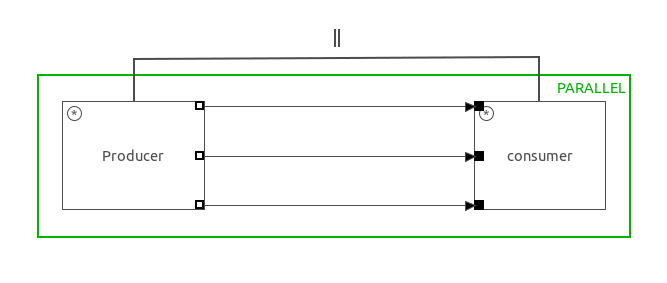
\includegraphics[scale=0.7]{./images/2-1_overview.png}
	 \caption{Overview diagram of the multiple channel producer consumer system.}
	 \label{fig:2_1-model:overview}
	\end{subfigure}
	\begin{subfigure}{0.5\textwidth}
		\centering
		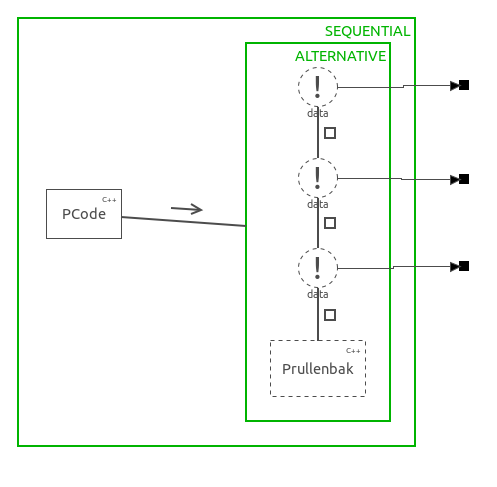
\includegraphics[width=\textwidth]{./images/2-1_producer.png}
		\caption{The producer process.}
		\label{fig:2_1-model:producer}
	\end{subfigure}%
	\begin{subfigure}{0.5\textwidth}
		\centering
		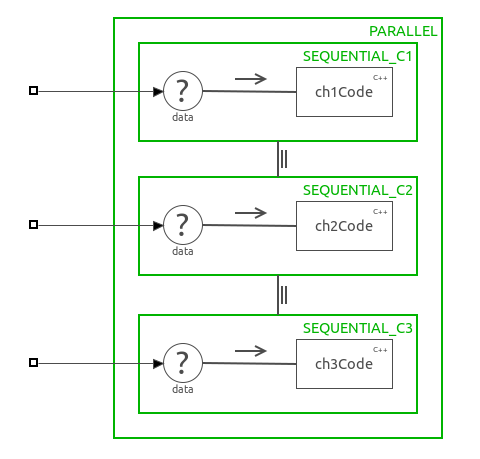
\includegraphics[width=\textwidth]{./images/2-1_consumer.png}
		\caption{The consumer process.}
		\label{fig:2_1-model:consumer}
	\end{subfigure}
	\caption{The CSP model of exercise 1.2.}
	\label{fig:2_1-model}
\end{figure}


\begin{figure}
	\centering
	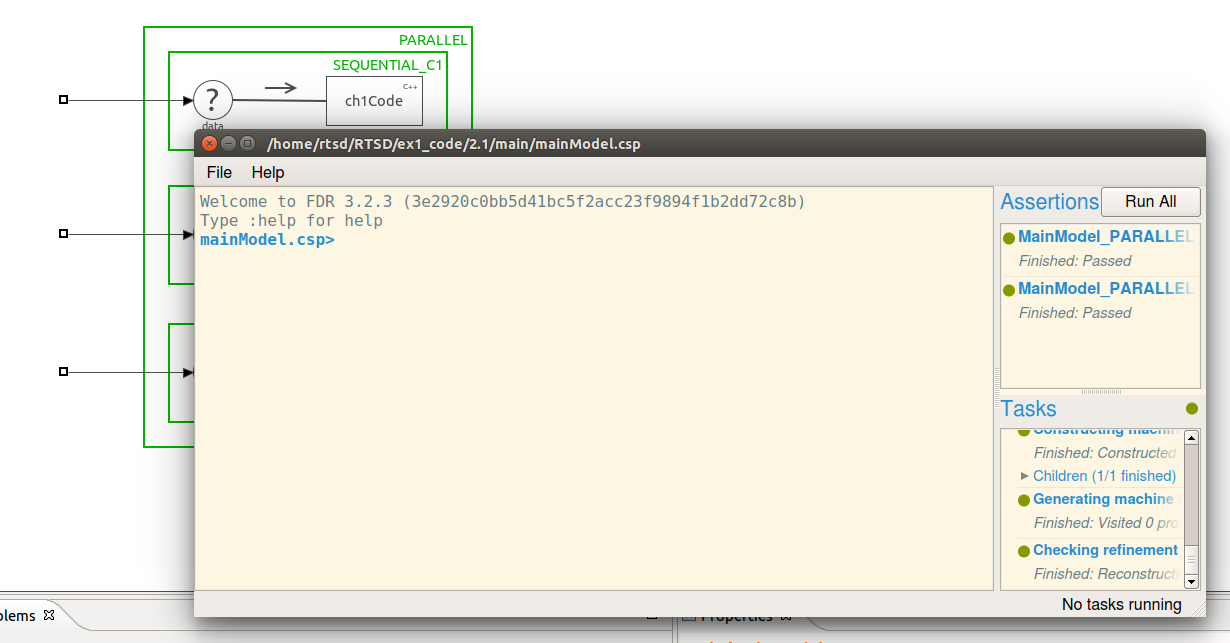
\includegraphics[width=\textwidth]{./images/2-1_fdr.png}
	\caption{Deadlock free.}
	\label{fig:2_1_DF}
\end{figure}

\begin{figure}
	\centering
	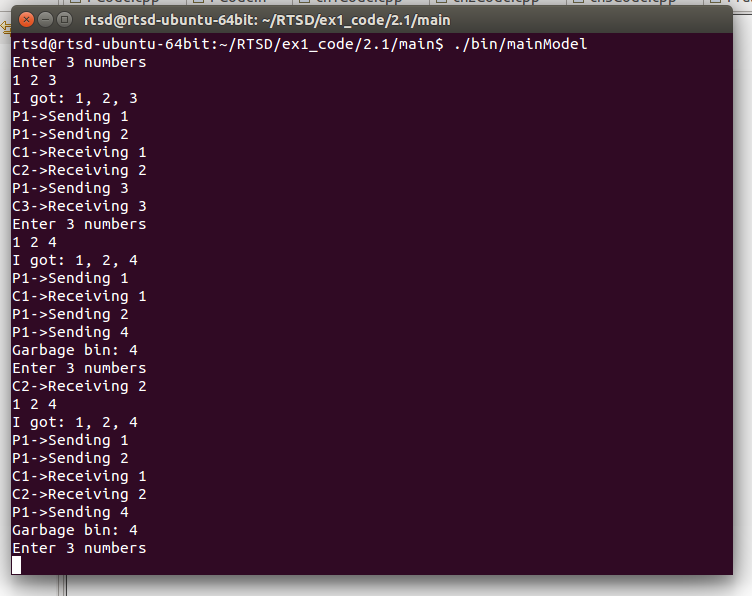
\includegraphics[width=\textwidth]{./images/2-1_output.png}
	\caption{Output of the program exercise 1.2.}
	\label{fig:2_1-output}
\end{figure}

\FloatBarrier
\subsection{}
\subsubsection{}
\begin{itemize}
	\item We simulated the execution of the model in 20-sim, results shown in figure~\ref{fig:3_1-simulation}.
		As expected, after $stepTime$ seconds, the input increases, and directly after $x$ increases with the value of the input $u$.
		After that we see $x$ increase again, but this time the increment is dampened by $x$ having a non-zero value.
		As $x$ increases, the increment decreases, until $u - 0.3x = 0 \Leftrightarrow x=\frac{10}{3}$.
		This equilibrium will, in theory, never be reached.
		In Figure~\ref{fig:3_1-simulation} we see $x$ reach a point between $3$ and $3.33...$.

	\item We recreated the 20-sim model in TERRA just to check for deadlocks.
		See Figure~\ref{fig:3_1_csp_model} for the models, and Figure~\ref{fig:3_1_csp_fdr} for a screenshot of FDR that proofs there are no deadlocks.

	\item We implemented the 20sim project into TERRA by using the 20sim LUNA template, editing the xml and importing 
		the 20sim models into the TERRA project after updating.
		See Figure~\ref{fig:3_1_terra_model} for the models of the TERRA project that includes \cpp code.
	\item Figure~\ref{fig:3_1_terra_output} shows the output of the control 
		loop program and Figure~\ref{fig:3_1-simulation} the output of the simulation.

		Note that the green line in the simulation (1.0) corresponds to the output of the setpoint value, and
		node that the blue line in the simulation (3.3) corresponds to the output of the steering value.

		The result of the program is the same as the simulation.
\end{itemize}
\textit{The configuration of the linear system is as follows:
\begin{align}
 x_n &= 1\cdot x+1 \cdot u\nonumber\\
 y   &= 1\cdot x+0 \cdot u\nonumber
\end{align}
where we use $u$ to for $dx$, calculated in the controller (see figure~\ref{fig:3_1-20sim-model:cont})}
\subsubsection{}
Figure~\ref{fig:3_2_model} depicts the model after implementing the new display 
process and Figure~\ref{fig:3_2_output} shows the output after running the TERRA 
\cpp program. Furthermore, Figure~\ref{fig:3_2_fdr} proofs that the program does not
deadlock.

We chose to have the display process to print only the steering value from the Controller
process and the setpoint value from the Step process.

\subsubsection{}
The e-mail of 28th of May stated that this exercise need not be implemented in TERRA.
\subsubsection{}
The e-mail of 28th of May stated that this exercise is not applicable in the 
current form, because exercise 1.3.3 need not be implemented.

\subsubsection{}
It is quite hard to truly test hard real-time constrains on a system that is not 
real time: the desktop PC that we use for executing TERRA programs is not real-time.

How do we know that hard-real-time constraints can always be met, and that the
soft-real-time and hard-real-time parts are always correctly executed, if the system itself is not real time? 

\subsubsection{}
Yes, the approach is still a very "sophisticated" way of working.
There are still several annoyances when using imported 20sim models in TERRA,
these might make the development of a large system very much more complex.

To name a few:
\begin{itemize}
	\item Imported 20sim models disable the use of CSP deadlock checking in FDR.
	\item Adding code to the \cpp files that are added by generated by imported 20sim 
		models cannot be saved (no protected areas).
	\item External models (imported 20sim models). Have to be generated separately.
\end{itemize}


\begin{figure}
	\centering
	\begin{subfigure}{0.5\textwidth}
	 \centering
	 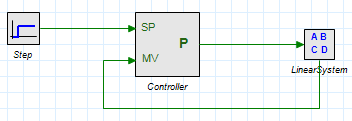
\includegraphics[width=\textwidth]{./images/3_1-20sim-model.png}
	 \caption{Model in 20-sim.}
	 \label{fig:3_1-20sim-model:model}
	\end{subfigure}%
	\begin{subfigure}{0.5\textwidth}
	 \centering
	 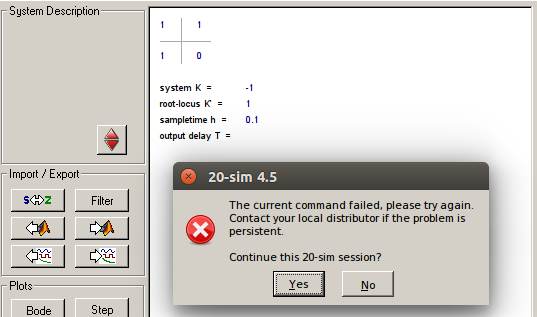
\includegraphics[width=\textwidth]{./images/3_1-20sim-plant.png}
	 \caption{Configuration of the linear system. Could not be fully shown because of a persistent error that crashes 20-sim.}
	 \label{fig:3_1-20sim-model:plant}
	\end{subfigure}
	\begin{subfigure}{0.5\textwidth}
	 \centering
	 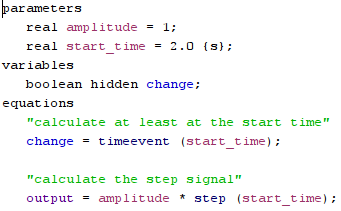
\includegraphics[width=\textwidth]{./images/3_1-20sim-model-stepfunction.png}
	 \caption{The definition of the step function.}
	 \label{fig:3_1-20sim-model:step}
	\end{subfigure}%
	\begin{subfigure}{0.5\textwidth}
	 \centering
	 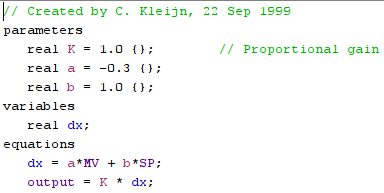
\includegraphics[width=\textwidth]{./images/3_1-20sim-model-controller.png}
	 \caption{The definition of the loop controller.}
	 \label{fig:3_1-20sim-model:cont}
	\end{subfigure}
	\caption{The model in 20 sim.}
	\label{fig:3_1-20sim-model}
\end{figure}

\begin{figure}
	\centering
	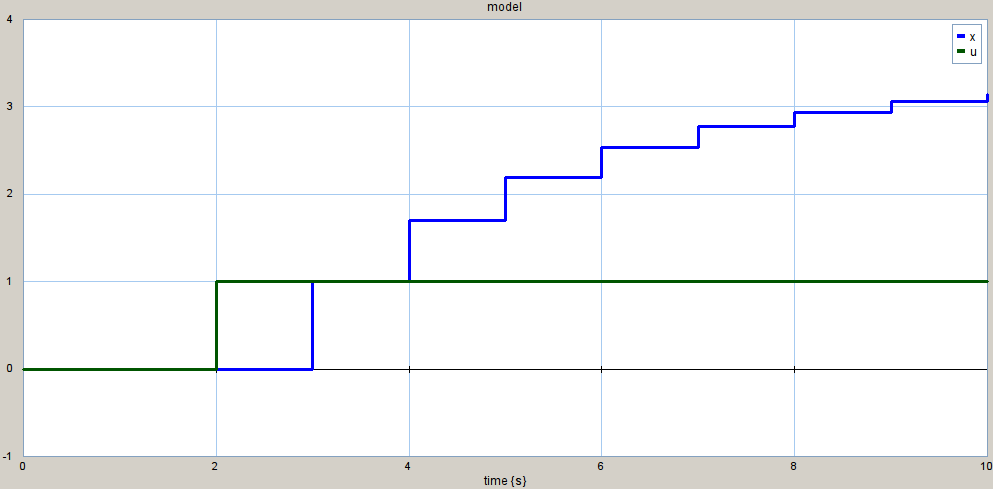
\includegraphics[width=\textwidth]{./images/3_1-simulation.png}
	\caption{Simulation in 20-sim of the model shown in figure~\ref{fig:3_1-20sim-model}. Blue line: $x$, green line: $u$.}
	\label{fig:3_1-simulation}
\end{figure}

\begin{figure}
	\centering
	\begin{subfigure}{0.5\textwidth}
	 \centering
	 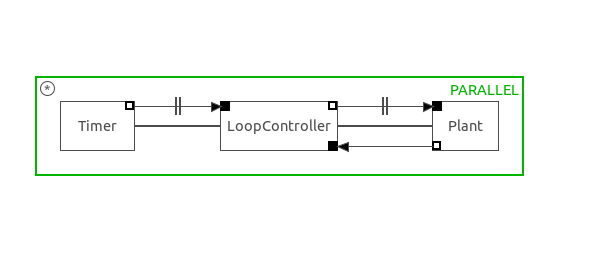
\includegraphics[width=\textwidth]{./images/3-1_csp_overview.png}
	 \caption{Control model in TERRA.}
	 \label{fig:3_1_csp_overview}
	\end{subfigure}%
	\begin{subfigure}{0.5\textwidth}
	 \centering
	 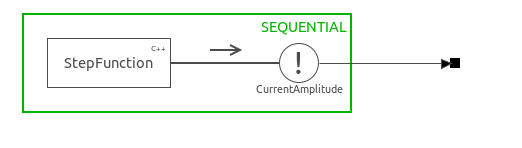
\includegraphics[width=\textwidth]{./images/3-1_csp_step.png}
	 \caption{Step controller (Timer)}
	 \label{fig:3_1_csp_step}
	\end{subfigure}
	\begin{subfigure}{0.5\textwidth}
	 \centering
	 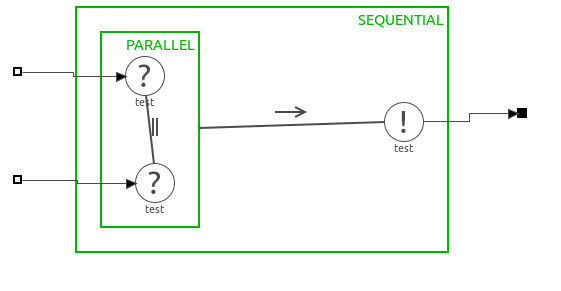
\includegraphics[width=\textwidth]{./images/3-1_csp_controller.png}
	 \caption{Loopcontroller.}
	 \label{fig:3_1_csp_controller}
	\end{subfigure}%
	\begin{subfigure}{0.5\textwidth}
	 \centering
	 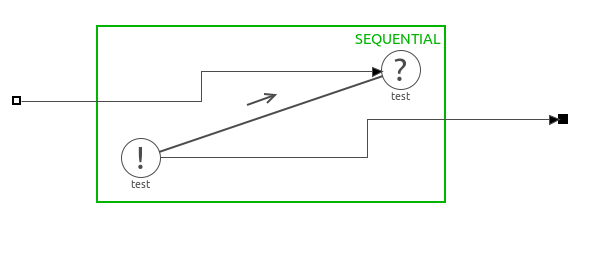
\includegraphics[width=\textwidth]{./images/3-1_csp_linearsystem.png}
	 \caption{LinearSystem (Plant)}
	 \label{fig:3_1_csp_linearsystem}
	\end{subfigure}
	\caption{Recreating the 20sim model to check for deadlocks.}
	\label{fig:3_1_csp_model}
\end{figure}

\begin{figure}
	\centering
	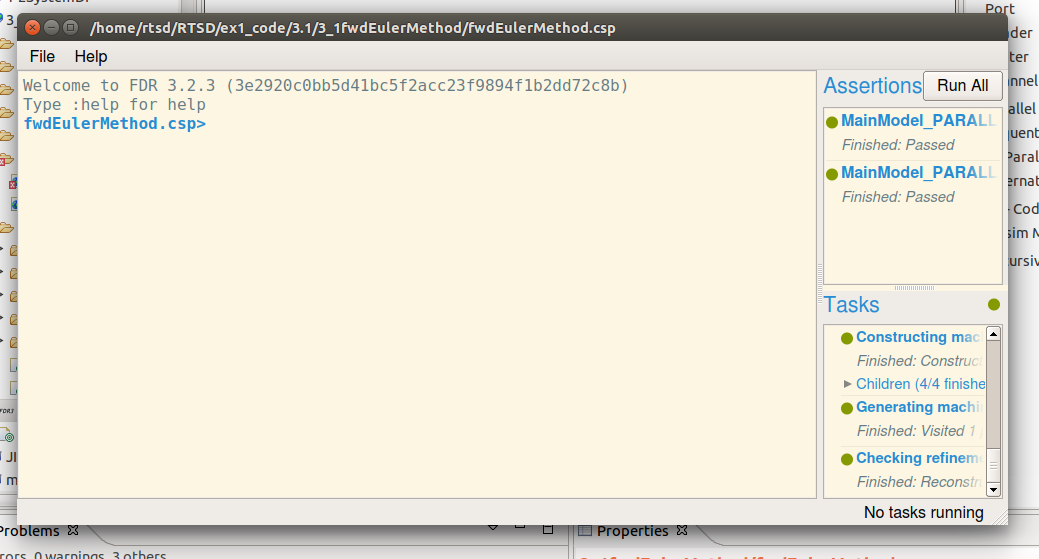
\includegraphics[width=\textwidth]{./images/3-1_csp_fdr.png}
	\caption{No deadlocks!}
	\label{fig:3_1_csp_fdr}
\end{figure}

\begin{figure}
	\centering
	\begin{subfigure}{0.5\textwidth}
	 \centering
	 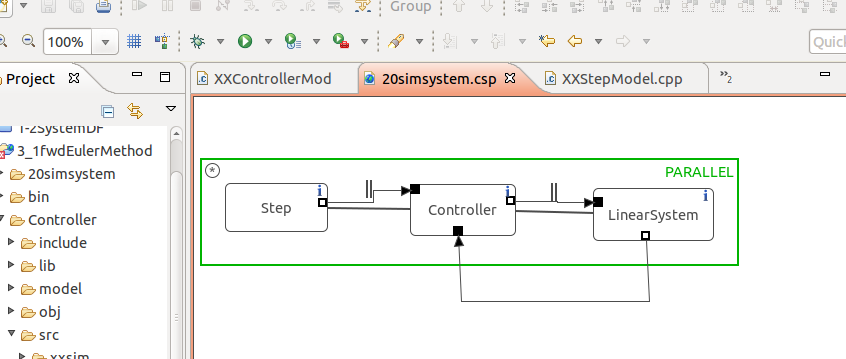
\includegraphics[width=\textwidth]{./images/3-1_terra_overview.png}
	 \caption{Control model in TERRA.}
	 \label{fig:3_1_terra_overview}
	\end{subfigure}%
	\begin{subfigure}{0.5\textwidth}
	 \centering
	 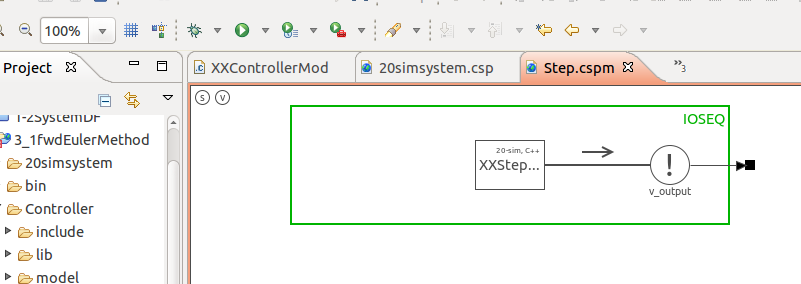
\includegraphics[width=\textwidth]{./images/3-1_terra_step.png}
	 \caption{Step controller (Step)}
	 \label{fig:3_1_terra_step}
	\end{subfigure}
	\begin{subfigure}{0.5\textwidth}
	 \centering
	 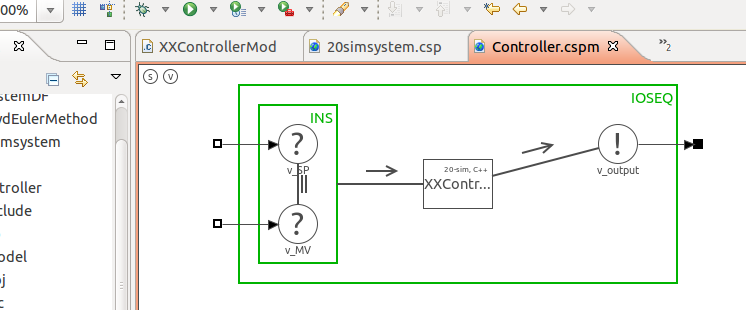
\includegraphics[width=\textwidth]{./images/3-1_terra_controller.png}
	 \caption{Loopcontroller (Controller).}
	 \label{fig:3_1_terra_controller}
	\end{subfigure}%
	\begin{subfigure}{0.5\textwidth}
	 \centering
	 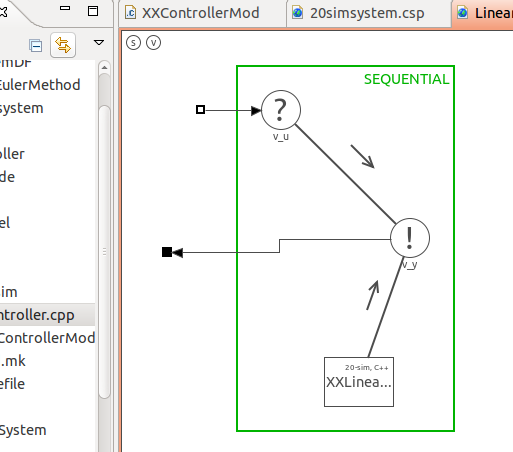
\includegraphics[width=\textwidth]{./images/3-1_terra_linearsystem.png}
	 \caption{Plant (LinearSystem)}
	 \label{fig:3_1_terra_linearsystem}
	\end{subfigure}
	\caption{Implementation of the control loop model with C++ code from 20sim.}
	\label{fig:3_1_terra_model}
\end{figure}

\begin{figure}
	\centering
	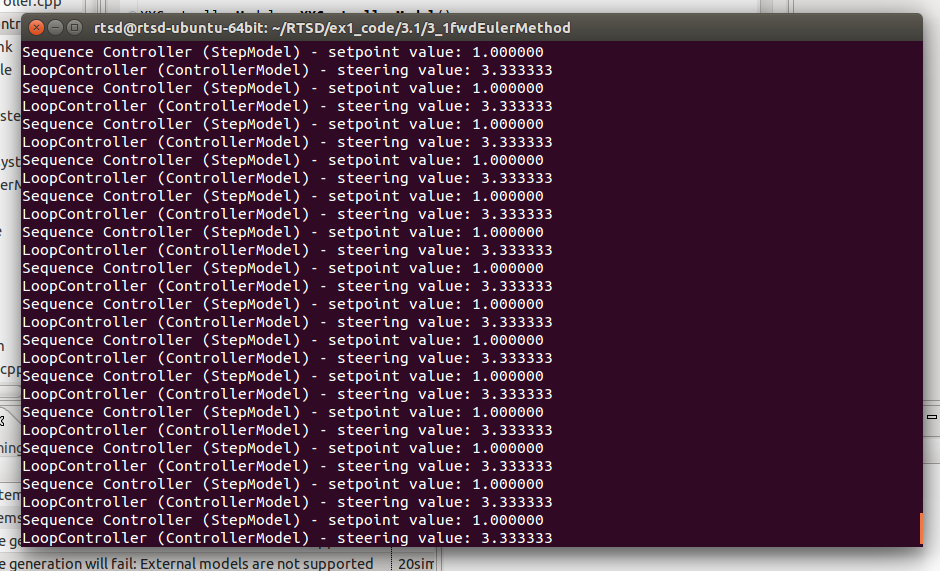
\includegraphics[width=\textwidth]{./images/3-1_terra_output.png}
	\caption{Output of the control loop model implemented in TERRA.}
	\label{fig:3_1_terra_output}
\end{figure}

\begin{figure}
	\centering
	\begin{subfigure}{0.6\textwidth}
	 \centering
	 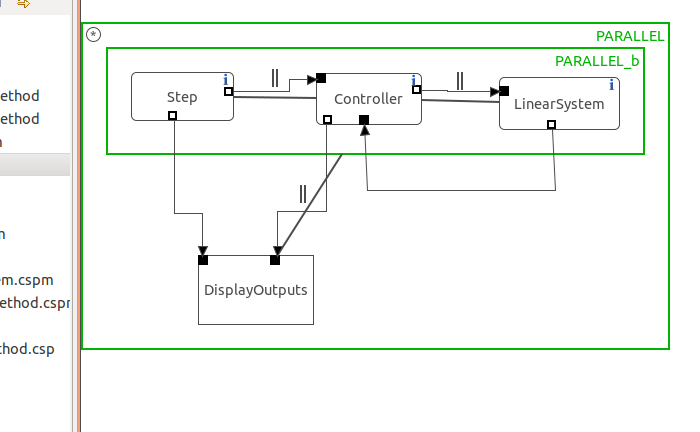
\includegraphics[width=\textwidth]{./images/3-2_overview.png}
	 \caption{Overview}
	 \label{fig:3_2_overview}
	\end{subfigure}%
	\begin{subfigure}{0.6\textwidth}
	 \centering
	 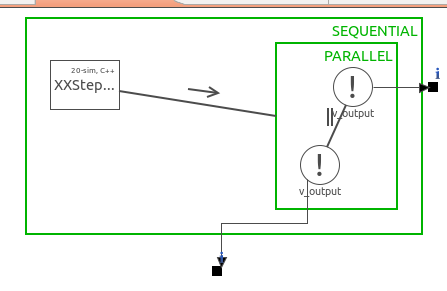
\includegraphics[width=\textwidth]{./images/3-2_step.png}
	 \caption{Step controller}
	 \label{fig:3_2_step}
	\end{subfigure}
	\begin{subfigure}{0.6\textwidth}
	 \centering
	 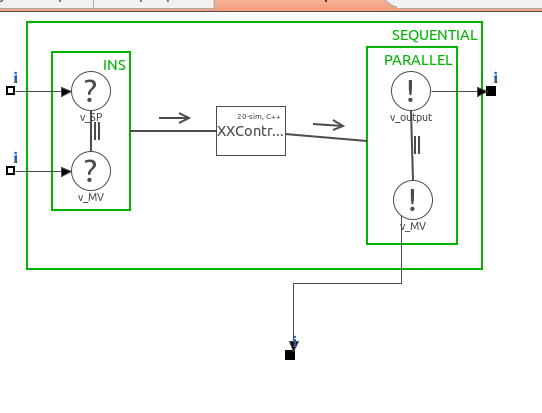
\includegraphics[width=\textwidth]{./images/3-2_controller.png}
	 \caption{Inside Controller }
	 \label{fig:3_2_controller}
	\end{subfigure}%
	\begin{subfigure}{0.6\textwidth}
	 \centering
	 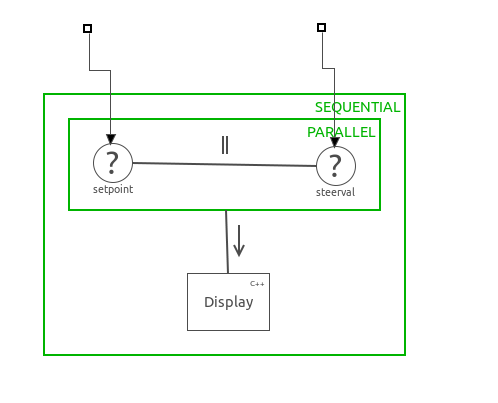
\includegraphics[width=\textwidth]{./images/3-2_display.png}
	 \caption{Inside the DisplayOutputs process.}
	 \label{fig:3_2_display}
	\end{subfigure}
	\caption{Separate Display process for printing values.}
	\label{fig:3_2_model}
\end{figure}

\begin{figure}
	\centering
	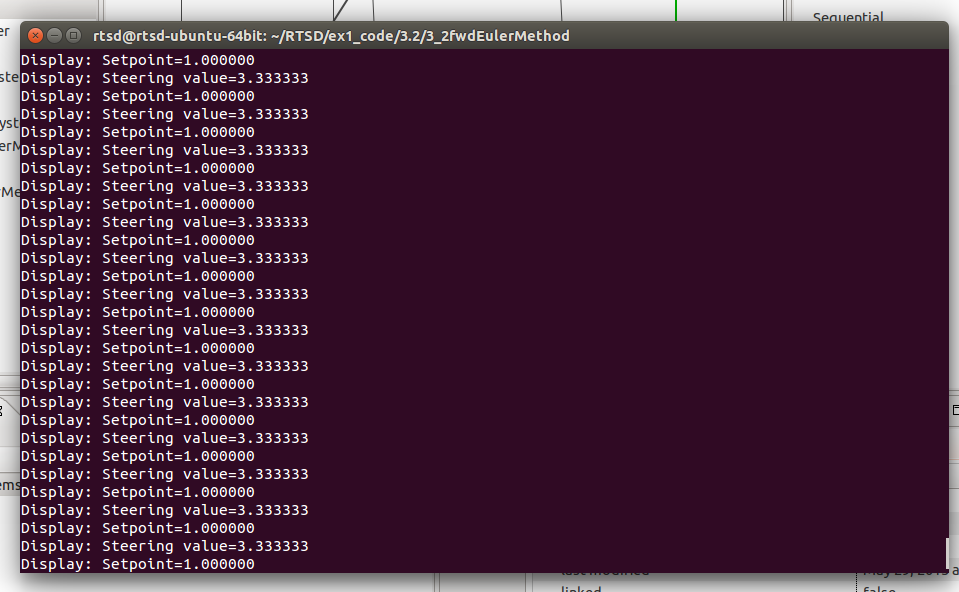
\includegraphics[width=\textwidth]{./images/3-2_output.png}
	\caption{Output of the separate display process (1.3.2)}
	\label{fig:3_2_output}
\end{figure}

\begin{figure}
	\centering
	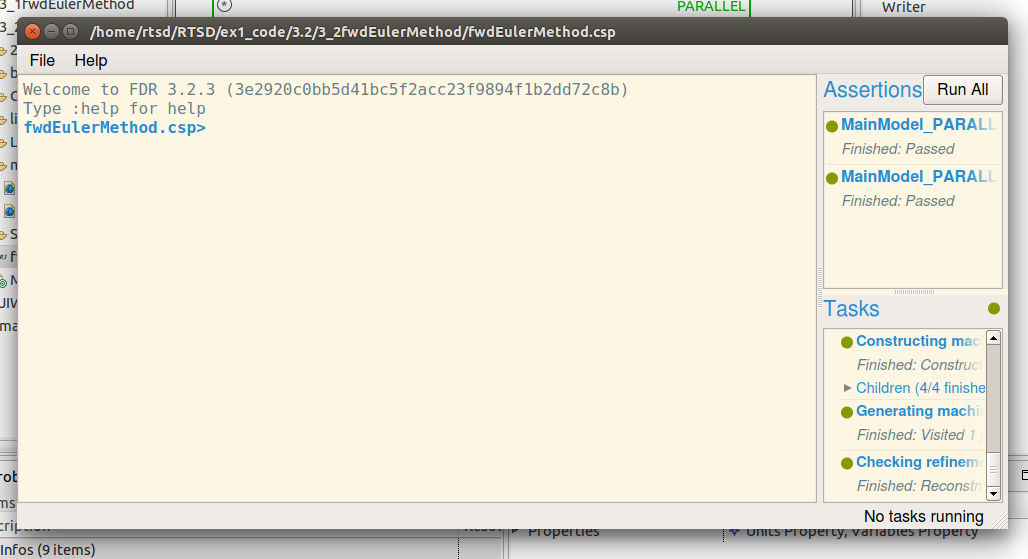
\includegraphics[width=\textwidth]{./images/3-2_fdr.png}
	\caption{After adding the display process we do not get any deadlocks.}
	\label{fig:3_2_fdr}
\end{figure}

\FloatBarrier
\subsection{}
\subsubsection{}
Figure~\ref{fig:4_1_model} presents the JIWY controller model as presented in 
the slides, with the addition of extra readers and writers that: simulate the 
input of the joystick, the output to the robot and the feedback from the robot.

This is added because otherwise it was not possible to generate CSPm: one 
cannot leave input and output ports unconnected in the top model.

Figure~\ref{fig:4_1_fdr} informs us that the model results in a deadlock in FDR.

\subsubsection{}
Figure~\ref{sub:4_2_check} shows the small fix to remove the deadlock and this 
is proven with a screenshot of FDR as seen in Figure~\ref{sub:4_2_fdr}. 

In the deadlock situation, observe the following:

\begin{itemize}
	\item The Check process must read from the Vertical process first,
		before it can read from the Horizontal process.

	\item The Vertical process must read from the Horizontal process before
	       	it can write to the Check process.

	\item The Horizontal process must first write to the Check process before 
		it can write to the Vertical process.
\end{itemize}
This results in the deadlock, we have a loop.
\smallskip

Making sure that the Check process has to read first from the Horizontal process 
instead of the Vertical process will fix the problem.

If the Check process first reads from the Horizontal process and then to the Vertical
process; the Horizontal Process is first able to write to the Check process and 
then to the Vertical process 
(which is waiting on Horizontal), and this in turn allows the Vertical process to write to the Check process.

The Check process is able to receive the write from the Vertical process because it first reads from Horizontal and then from Vertical.

\smallskip
So this small change fixes the deadlock, see Figure~\ref{sub:4_2_check}.
Note the arrow is actually in the wrong direction, this is a visual bug in TERRA.

\begin{figure}
	\begin{subfigure}{0.5\textwidth}
		\centering
		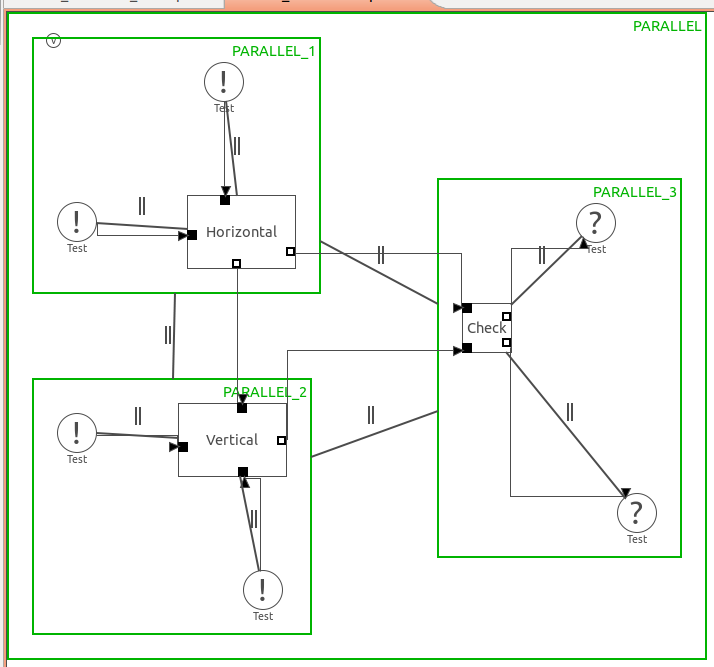
\includegraphics[width=\textwidth]{./images/4-1_overview.png}
		\caption{Overview diagram of JIWY model.}
		\label{sub:4_1_overview}
	\end{subfigure}%
	\begin{subfigure}{0.5\textwidth}
		\centering
		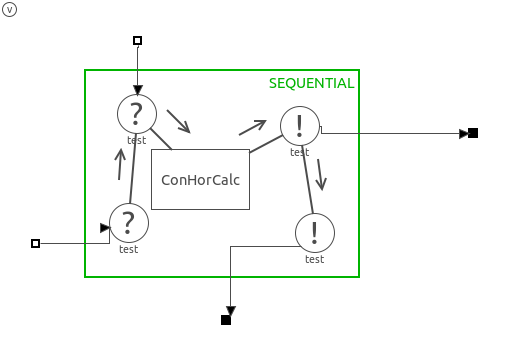
\includegraphics[width=\textwidth]{./images/4-1_hor.png}
		\caption{Inside the Horizontal process.}
		\label{sub:4_1_hor}
	\end{subfigure}%

	\begin{subfigure}{0.5\textwidth}
		\centering
		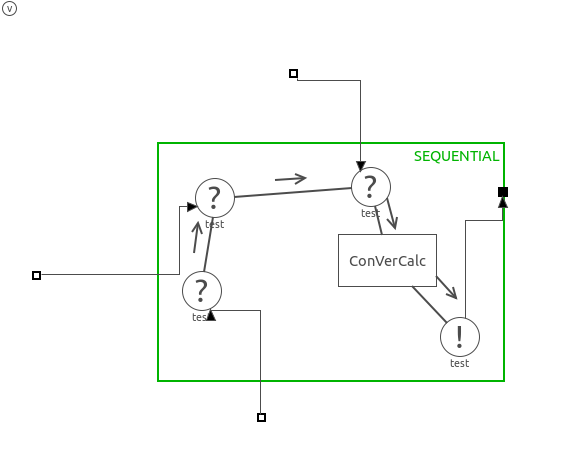
\includegraphics[width=\textwidth]{./images/4-1_ver.png}
		\caption{Inside the Vertical process.}
		\label{sub:4_1_vert}
	\end{subfigure}
	\begin{subfigure}{0.5\textwidth}
		\centering
		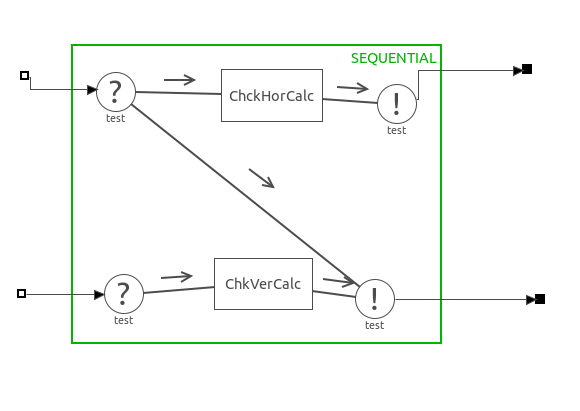
\includegraphics[width=\textwidth]{./images/4-1_contr.png}
		\caption{Inside the Check process.}
		\label{sub:4_1_check}
	\end{subfigure}
	\caption{JIWY controller model (deadlock).}
	\label{fig:4_1_model}
\end{figure}

\begin{figure}
	\centering
	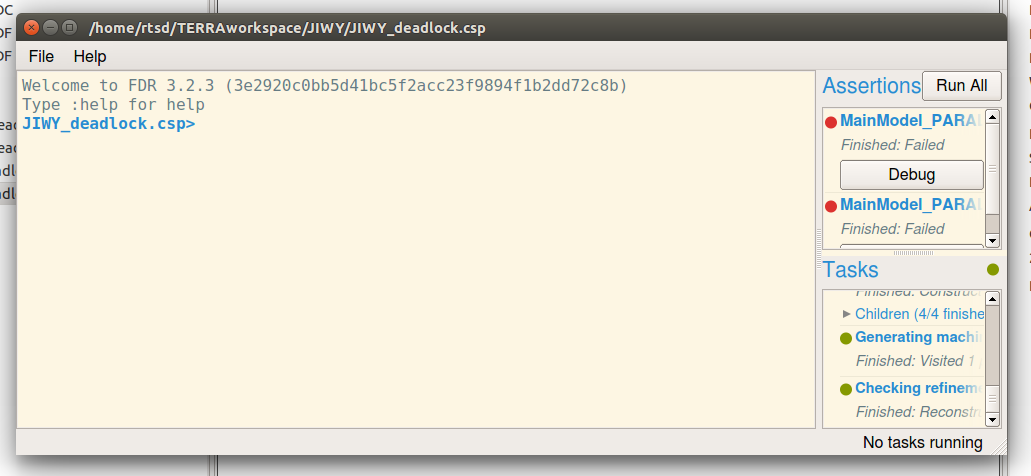
\includegraphics[width=\textwidth]{./images/4-1_fdr.png}
	\caption{The model deadlocks.}
	\label{fig:4_1_fdr}
\end{figure}

\begin{figure}
	\begin{subfigure}{0.6\textwidth}
		\centering
		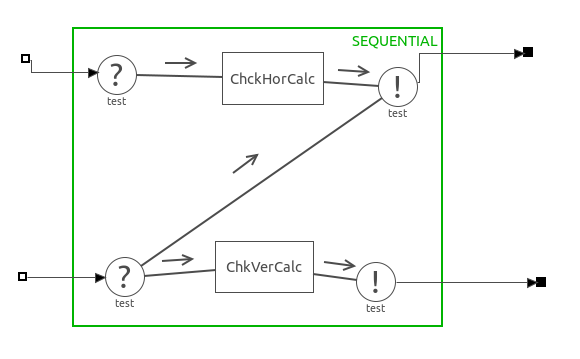
\includegraphics[width=\textwidth]{./images/4-2_contr.png}
		\caption{Minimal deadlock fix.}
		\label{sub:4_2_check}
	\end{subfigure}

	\begin{subfigure}{0.8\textwidth}
		\centering
		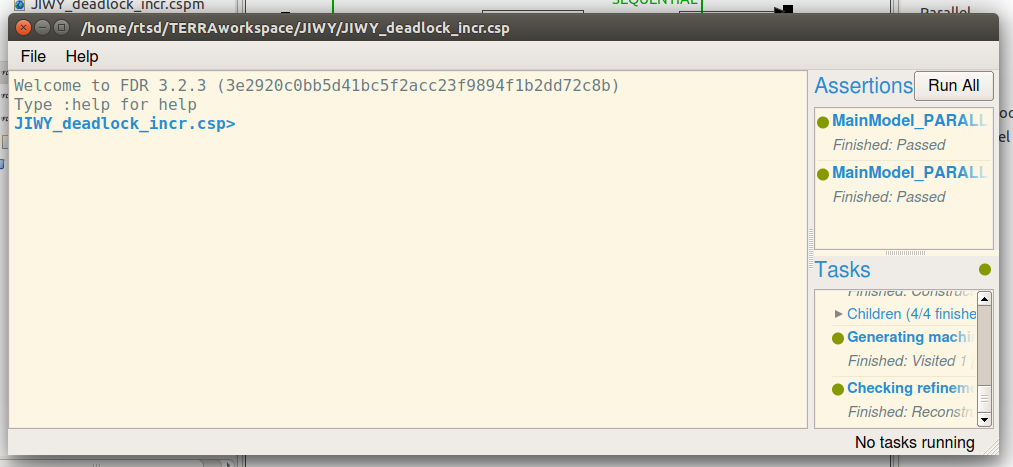
\includegraphics[width=\textwidth]{./images/4-2_fdr.png}
		\caption{No deadlock according to FDR.}
		\label{sub:4_2_fdr}
	\end{subfigure}
	\caption{Fixing the deadlock.}
\end{figure}
\begin{figure}
	\begin{subfigure}{0.6\textwidth}
		\centering
		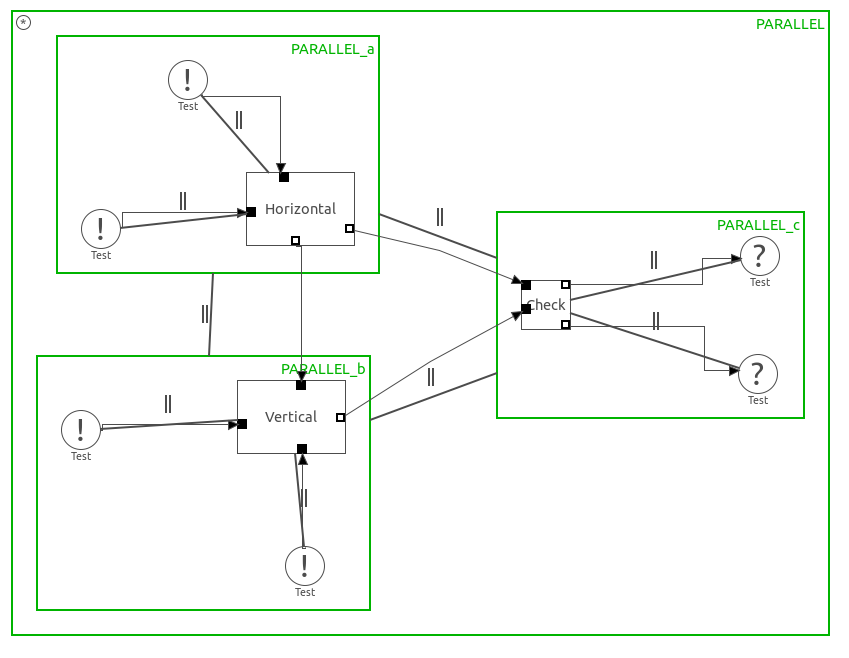
\includegraphics[width=\textwidth]{./images/4-3_overview.png}
		\caption{Overview diagram of JIWY model.}
		\label{sub:4_3_overview}
	\end{subfigure}%
	\begin{subfigure}{0.6\textwidth}
		\centering
		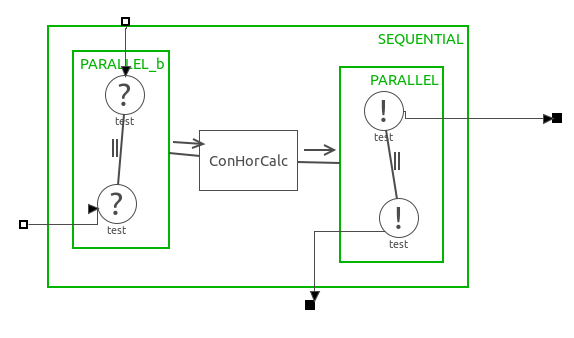
\includegraphics[width=\textwidth]{./images/4-3_hor.png}
		\caption{Inside the Horizontal process.}
		\label{sub:4_3_hor}
	\end{subfigure}%

	\begin{subfigure}{0.6\textwidth}
		\centering
		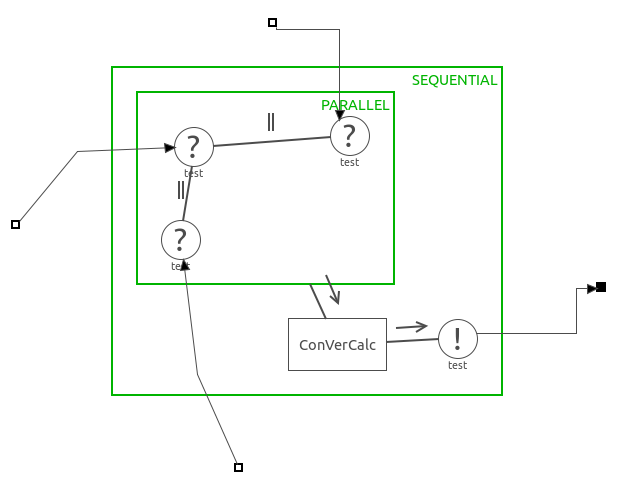
\includegraphics[width=\textwidth]{./images/4-3_ver.png}
		\caption{Inside the Vertical process.}
		\label{sub:4_3_vert}
	\end{subfigure}
	\begin{subfigure}{0.6\textwidth}
		\centering
		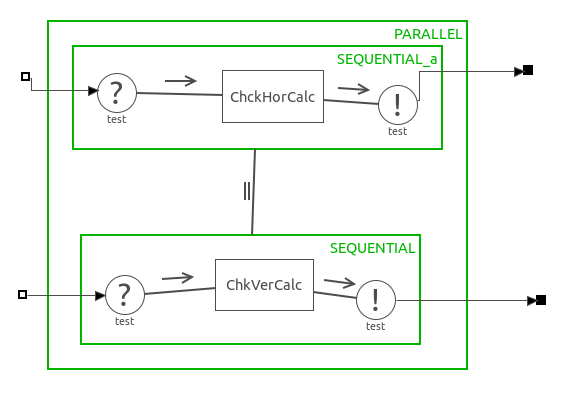
\includegraphics[width=\textwidth]{./images/4-3_check.png}
		\caption{Inside the Check process.}
		\label{sub:4_3_check}
	\end{subfigure}
	\caption{JIWY controller model IO SEQ pattern.}
	\label{fig:4_3_model}
\end{figure}

\begin{figure}
	\centering
	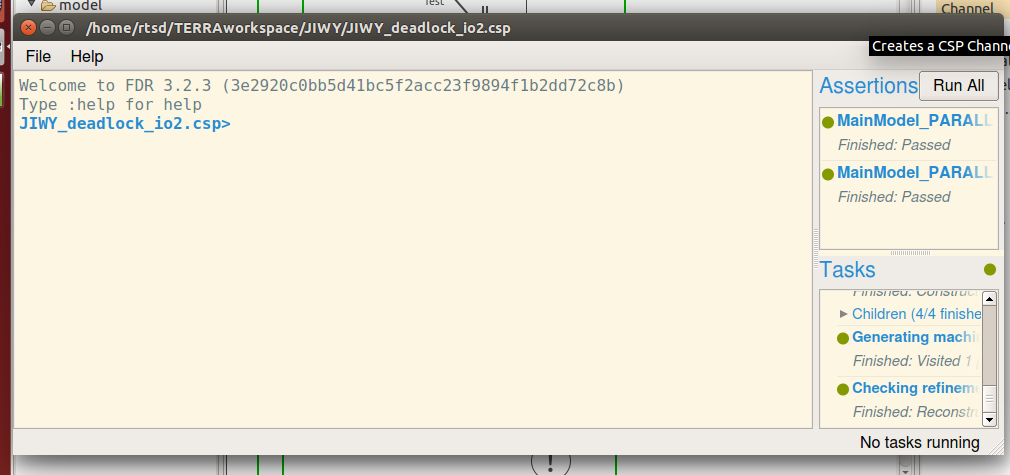
\includegraphics[width=\textwidth]{./images/4-3_fdr.png}
	\caption{No deadlock with the IO SEQ pattern.}
	\label{fig:4_3_fdr}
\end{figure}

\subsubsection{}
Figure~\ref{fig:4_3_model} shows the IO SEQ pattern used on the JIWY model and 
Figure~\ref{fig:4_3_fdr} displays the output of FDR, which does not deadlock.

\subsubsection{}
Figure~\ref{fig:4_4_model} presents the TERRA system that we made to test the JIWY\_Controller.

Figure~\ref{sub:4_4_controller} shows us the JIWY controller model with unconnected inputs and outputs that is being tested,
and Figure~\ref{sub:4_4_overview} depicts a higher level of the system with JIWY\_Controller model of Figure~\ref{sub:4_4_controller} as a process.  

Figure~\ref{fig:4_4_fdr} proofs that the model is deadlock free.

\begin{figure}
	\begin{subfigure}{0.5\textwidth}
		\centering
		\includegraphics[width=\textwidth]{./images/4-4_overview.png}
		\caption{JIWY\_Controller is "under test".}
		\label{sub:4_4_overview}
	\end{subfigure}
	\begin{subfigure}{0.6\textwidth}
		\centering
		\includegraphics[width=\textwidth]{./images/4-4_controller.png}
		\caption{Inside the JIWY\_Controller process.}
		\label{sub:4_4_controller}
	\end{subfigure}
	\caption{"Submodel under test".}
	\label{fig:4_4_model}
\end{figure}

\begin{figure}
	\centering
	\includegraphics[width=\textwidth]{./images/4-4_fdr.png}
	\caption{No deadlock with model under test TERRA System.}
	\label{fig:4_4_fdr}
\end{figure}

\subsubsection{}
The solution of 1.4.2 expects that data will always be available from the inputs 
to the model, and if this is not the case then the system waits until data is written, 
because of the sequential reader-writer structure.

Solution 1.4.3 does not have this problem because the inputs and outputs are in parallel.

So, having the inputs/outputs in parallel is the main advantage of 1.4.3.

\subsubsection{}
One might choose to use the JIWY\_Controller model in other TERRA systems, where only the input and outputs are different.

If you use the ``submodel under test'' approach you clearly separate the model and you make the interfaces to the model more clear.

In the case of large models with a lot of inputs and outputs, in can become very confusing if you need to change all the inputs/outputs from temporary test inputs/outputs (readers/writers) to say, \cpp code blocks.

\subsubsection{}
The method of using ``simple generator submodels'' and ``readers in the submodel 
that consumes the outputs'' assumes that there is always incoming data to the model and always a possibility that output data of the model can be read.

In its realization, however, problems might occur if the system does not get input at all, or if the output buffers are full.

Implementing \cpp code blocks that simulate reading and writing,
but with momentary (random) intervals of pausing, might more closely resemble a real feedback-control system.

\end{document}
